\documentclass[12pt,a4]{article}

\usepackage{pythonhighlight}

\author{Yujie Lu \quad Jiabao Ji \quad Tong Chen}
\newtheorem{thm}{Theorem}
\newtheorem{pro}{Problem}
\newtheorem{defi}{Definition}
\newtheorem{li}{Example}
\newenvironment{proof}{\paragraph{Proof:}}{\hfill$\square$}
\newenvironment{jie}{\paragraph{Show:}}{\hfill$\square$}



\newcommand{\handoutdate}{Monday, 2020-03-23}
\newcommand{\firstduedate}{Friday, 2020-03-27}
\newcommand{\finalduedate}{Friday, 2020-04-04}




\usepackage{graphicx,amsmath,amssymb,amsthm, boxedminipage}



\usepackage{algorithm}
\usepackage{algpseudocode}


\newtheorem{theorem}{Theorem}%[section]
\newtheorem{proposition}[theorem]{Proposition}
\newtheorem{lemma}[theorem]{Lemma}
\newtheorem{corollary}[theorem]{Corollary}
\newtheorem{definition}[theorem]{Definition}



\newcommand{\scalar}[2]{\ensuremath{\langle #1, #2\rangle}}
\newcommand{\floor}[1]{\left\lfloor #1 \right\rfloor}
\newcommand{\ceil}[1]{\left\lceil #1 \right\rceil}
\newcommand{\norm}[1]{\|#1\|}
\newcommand{\pfrac}[2]{\left(\frac{#1}{#2}\right)}
\newcommand{\nth}[1]{#1\textsuperscript{th}}

% \newcommand{\nth}[1]{#1\textsuperscript{th}}
\newcommand{\E}{\mathop{\mathbb{E\/}}}
\newcommand{\N}{\mathbb{N}}

\newcommand{\R}{\mathbb{R}}

\newtheorem{exercise}[theorem]{Exercise}
\newtheorem{exerciseD}[theorem]{*Exercise}
\newtheorem{exerciseDD}[theorem]{**Exercise}

\let\oldexercise\exercise
\renewcommand{\exercise}{\oldexercise\normalfont}

\let\oldexerciseD\exerciseD
\renewcommand{\exerciseD}{\oldexerciseD\normalfont}

\let\oldexerciseDD\exerciseDD
\renewcommand{\exerciseDD}{\oldexerciseDD\normalfont}


 
\begin{document}

\date{}

\title{CS 217 -- Algorithm Design and Analysis \\ 
  \vspace{3mm}
{\large	Shanghai Jiaotong University, Fall 2019\\
}
}
\maketitle

\noindent
Handed out on \handoutdate{}\\
First submission and questions due on \firstduedate{}\\
You will receive feedback from the TA.\\
Final submission due on \finalduedate{}



\setcounter{section}{1}


\section{Sorting Algorithms}

\begin{exercise}
   Given an array $A$ of $n$ items (numbers), we can find the maximum with $n-1$ comparisons (this is simple).
   Show that this is optimal: that is, any algorithm that does $n-2$ or fewer comparisons will fail to find the maximum 
   on some inputs.
\end{exercise}
\begin{proof}
Prove it by induction on the length of array, denote the length as $n$ and elements $a_i(1 \leq i \leq n)$.\\
$Base: n = 1$\\
    \hspace*{1em}Obviously, $a_1$ itself is the maximal element, no comparison is needed at all.\\
$Induction: n = k \rightarrow n = k + 1$
    As for $a_1, a_2, ... , a_{k}$, the minimal comparison it takes is $k - 1$, by induction hypothesis.
    Suppose the maximal element in $a_1...a_{k}$ is $b$, since we don't know whether $b > a_k$, we have to
    do another comparison. In all, we do $k - 1 + 1 = k$ comparisons for $n = k + 1$. 
\end{proof}

\begin{exercise}
  Let $A$ be an array of size $n$, where $n$ is even. 
  Describe how to find both the minimum and the maximum
  with at most $\frac{3}{2} n  - 2$ comparisons.
  Make sure your solution is {\em simple}, in describe it 
  in a clear and succinct way!
\end{exercise}
\begin{proof}
\begin{python}
    def ComputeMaxMin(A):
        # A is an array with n = 2m elements
        n = len(A)
        m = n // 2
        MinCandidate = []
        MaxCandidate = []
        for i in range(m):
            x = A[2 * i]
            y = A[2 * i + 1]
            if (x < y):
                MinCandidate.append(x)
                MaxCandidate.append(y)
            else:
                MinCandidate.append(y)
                MaxCandidate.append(x)
        
        Min = sys.maxint
        Max = -sys.maxint
        for i in range(m):
            if MinCandidate[i] < Min:
                Min = MinCandidate[i]
            if MaxCandidate[i] > Max:
                Max = MaxCandidate[i]
        return Min, Max
\end{python}
    \hspace*{1em} Based on the algorithm above, we can get the minimal element and maximal element in the $n$ items
    with exactly $\frac{3}{2} n - 2$ comparisons.\\
    \hspace*{1em} Since the array has $n = 2m$ elements, we can first compare any consecutive two elements in the array
    for $m$ times to divide the original array into two subarray as $MaxCandidate$, $MinCandidate$. We know for sure that
    maximal element is in $MaxCandidate$ and minimal element is in $MinCandidate$.\\
    \hspace*{1em} Using the result in  $Exer.1$, we need $m - 1$ times of comparisons to get minimal element form $MinCandidate$
    and another $m - 1$ comparisons for maximal. In all, we do $m + m - 1 + m - 1 = 3m-2 =\frac{3}{2}n - 2$ comparisons.
\end{proof}

\begin{exercise}
  Given an array $A$ of size $n = 2^k$, find the second largest element element
  with at most $n + \log_2(n)$ comparisons. 
  Again, your solution should be {\em simple}, and you should explain
  it in a clear and succinct way!
\end{exercise}
\begin{proof}
    \subsection*{Exer.3:}
    \begin{python}
    class Node:
        def __init__(self, weight, father, biggerSon, smallerSon):
            self.weight = weight
            self.father = father
            self.biggerSon = biggerSon
            self.smallerSon = smallerSon
    
    def ComputeSecondMax(A):
            # A should be an array with 2^k elements
            comparisons = 0
            n = len(A)
            k = math.floor(math.log(n, 2))
            MaxCandidate = []
            for x in A:
                MaxCandidate.append(Node(x, None, None, None))
            for _ in range(k):
                tmpMaxCandidate = []
                for j in range(len(MaxCandidate) // 2):
                    x = MaxCandidate[2 * j]
                    y = MaxCandidate[2 * j + 1]
                    if (x.weight < y.weight):
                        comparisons += 1
                        newNode = Node(y.weight, None, y, x)
                        tmpMaxCandidate.append(newNode)
                        x.father = newNode
                        y.father = newNode
                    else:
                        comparisons += 1
                        newNode = Node(x.weight, None, x, y)
                        tmpMaxCandidate.append(newNode)
                        x.father = newNode
                        y.father = newNode
                MaxCandidate = tmpMaxCandidate
    
            res = 0
            curNode = MaxCandidate[0]
            for _ in range(k):
                if curNode.smallerSon.weight > res :
                    res = curNode.smallerSon.weight
                    comparisons += 1
                comparisons += 1
                curNode = curNode.biggerSon
            return comparisons, res
    \end{python}
        \hspace*{1em} The algorithm is similar to the one in $Exer.2$, we can divide the original array for $k$ times, each time, we 
        get the bigger element from consecutive 2 elements in the last iteration. The array size is $2^k, 2^{k - 1}...2^{1}$
        And it takes $2^i - 1$ comparisons for $2^i$ size array. But to get the second max element we still need to do something else.
        \newpage
        \begin{figure}[h]
            \centering
            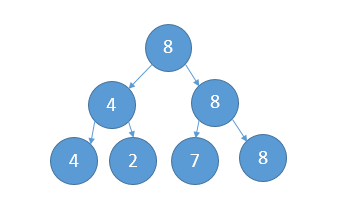
\includegraphics[]{2-wayTree.png}
            \caption{Comparing Tree in Exer.3}
        \end{figure}
        \hspace*{1em}After $k$ iterations of comparing consecutive elements, we constructed the comparing tree above.
        Obviously, the maximal element floats up from bottom to top, and the candidates for second maximal element
        are those who once compared to the maximal element in the tree, 4 and 7 in above specific tree, for example.\\
        \hspace*{1em}So we need to compare another $log_2(n) - 1$ times to get the maximal element in the candidates since maximal element 
        needs to be compared for $log_2(n)$ times to float to top.\\
        \hspace*{1em}In all we do $1 + 2 + 2^2 +... + 2^{k - 1} + log_2(n) = n + log_2(n)$ comparisons.\\
    
\end{proof}

Recall the quicksort tree defined in the lecture.
 \begin{center}
 	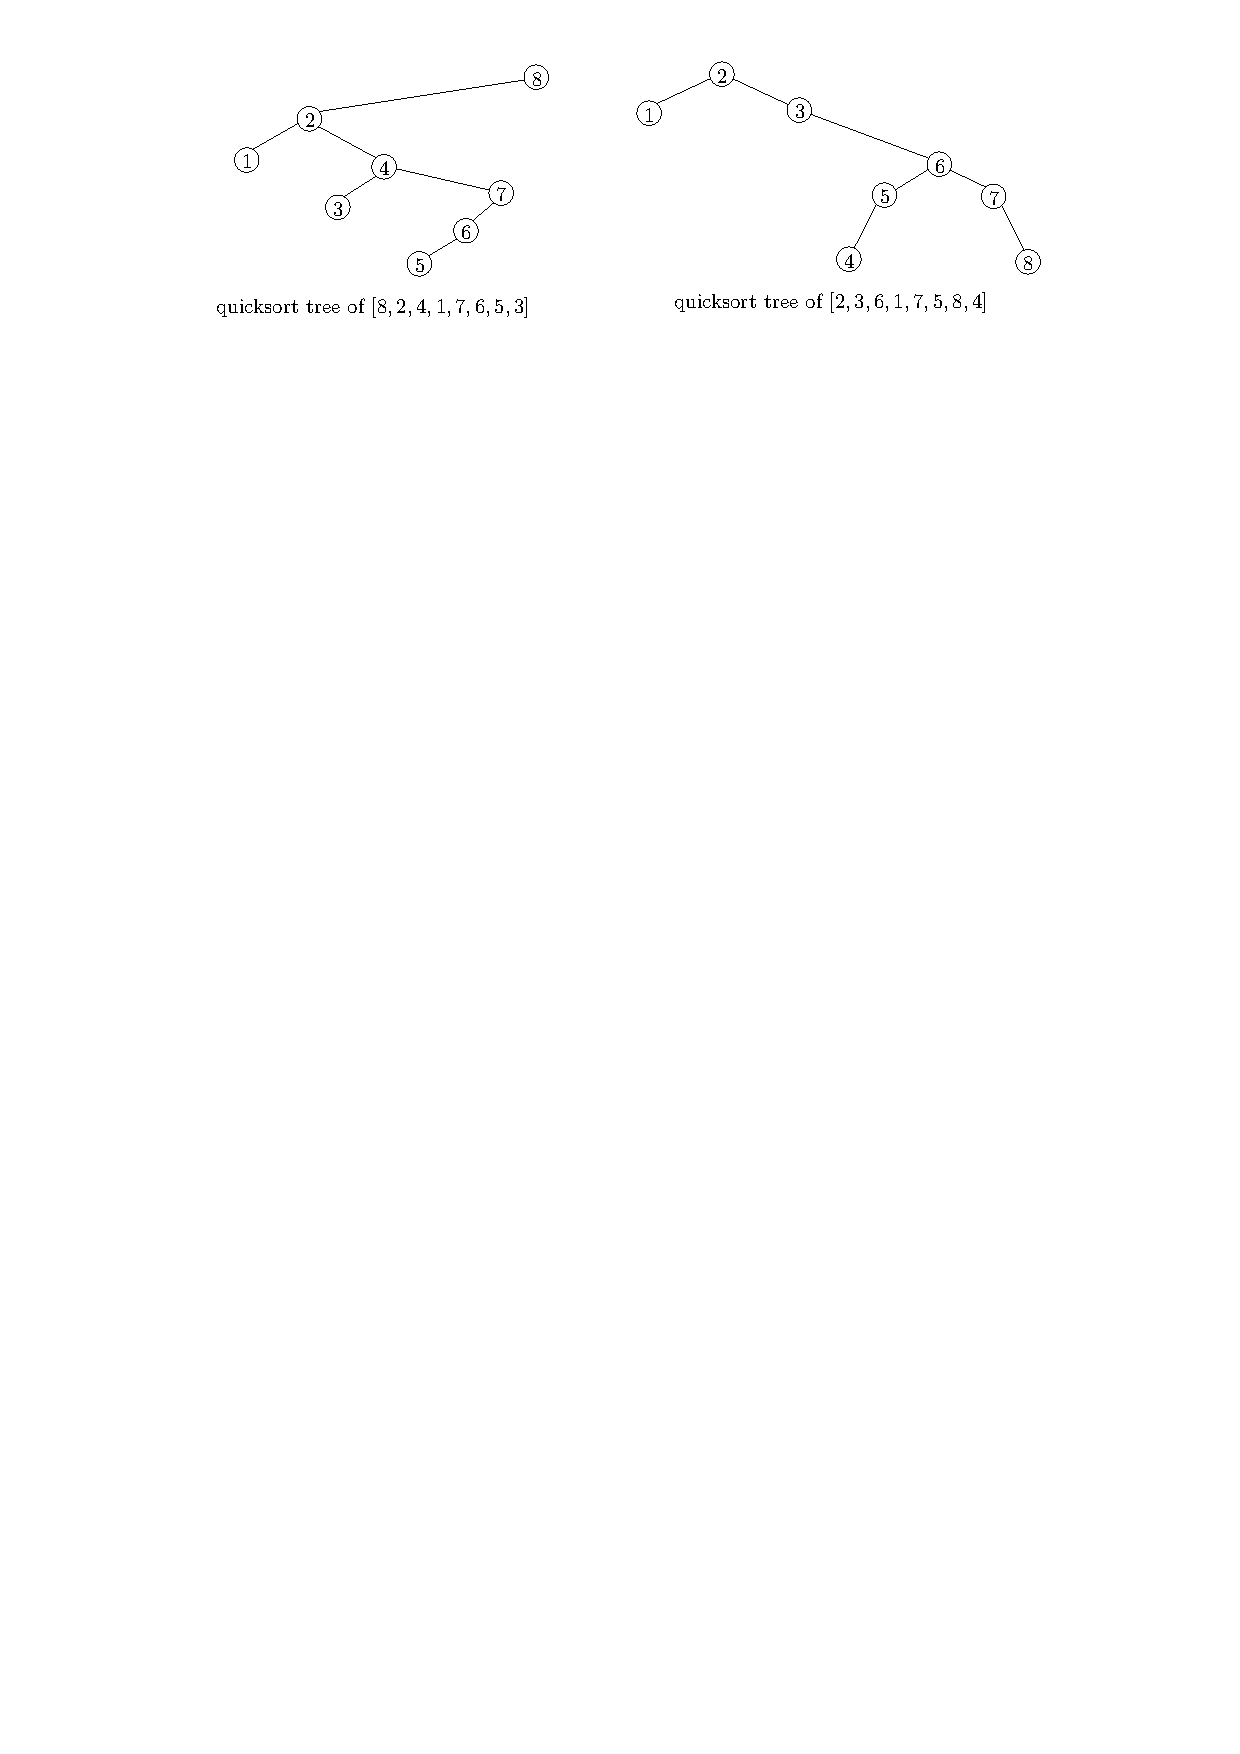
\includegraphics[width=\textwidth]{figures/quicksort-tree.pdf}
\end{center}
\begin{proof}
\begin{python}
    def ComputeSecondMax(A):
        # A should be an array with 2^k elements
        n = len(A)
        k = math.floor(math.log(n, 2))
        MaxCandidate = A
        for _ in range(k):
            tmpMaxCandidate = []
            for j in range(len(MaxCandidate) // 2):
                x = MaxCandidate[2 * j]
                y = MaxCandidate[2 * j + 1]
                if (x < y):
                    tmpMaxCandidate.append(y)
                else:
                    tmpMaxCandidate.append(x)
            MaxCandidate = tmpMaxCandidate
        return MaxCandidate[0]
\end{python}
    The algorithm is similar to the one in $Exer.2$, we can divide the original array for $k$ times, each time, we 
    get the bigger element from consecutive 2 elements in the last iteration. The array size is $2^k, 2^{k - 1}...2^{1}$
    And it takes $2^i - 1$ comparisons for $2^i$ size array.
    In all we do $1 + 2 + 2^2 +... + 2^{k - 1} = 2^k = n$ comparisons.\\
    FixMe: 存疑。。
\end{proof}

We denote a specific list (ordering) by $\pi$ and the tree by $T(\pi)$. $A_{i,j}$ is an indicator
variable which is $1$ if $i$ is an ancestor of $j$ in the tree $T(\pi)$, and $0$ otherwise.
In the lecture, we have derived:
\begin{align*}
	\E[A_{i,j}] & = \frac{1}{|i-j|+1} \\
	\textnormal{ total number of comparisons } & = \sum_{i \ne j} A_{i,j} \ . 
\end{align*}


\begin{exercise}
 Determine the expected number of comparisons made by quicksort. 
 Your final formula must be {\em closed}, meaning it must not contain 
 $\E$, $\prod$, or $\sum$. It may, however, contain $H_n := 1 + \frac{1}{2} + \frac{1}{3} + 
 \dots + \frac{1}{n}$ , the 
 $\nth{n}$ Harmonic number. \textbf{Remark.} This gets a bit tricky, and you will need some
 summation wizardry towards the end.
 \end{exercise}
 \begin{proof}
From the sum equation in the class, we can derive the result as follows.
\begin{align*}
    \mathbb{E}  & = \sum_{i \neq j} \frac{1}{|i - j| + 1}\\
                & = 2\sum_{1 \leq i < j \leq n} \frac{1}{j - i + 1}\\
                & = 2(\frac{1}{1 + 1}(n - 1) + \frac{1}{2 + 1}(n - 2) + ... + \frac{1}{n - 1 + 1}(n - (n - 1)))\\
                & = 2(\frac{1}{2}n + \frac{n}{3} + ... + \frac{n}{n} - (\frac{1}{2} + \frac{2}{3} + ... + \frac{n - 1}{n}))\\
                & = 2(n(\frac{1}{2} + ... + \frac{1}{n}) - (1 - \frac{1}{2}) - (1 - \frac{1}{3}) -... - (1 - \frac{1}{n}))\\
                & = 2(n(H_n - 1) - (n - 1) + (H_n -1))\\
                & = 2((n + 1)H_n - 2n)\\
                & = 2nH_n + 2H_n - 4n
\end{align*}
 \end{proof}

\subsection{Quickselect}

Remember the recursive algorithm \textsc{QuickSelect} from the lecture. I write
it below in pseudocode. In analogy to quicksort we define QuickSelect deterministically
and assume that the input array is random, or has been randomly shuffled before
QuickSelect is called. We assume that $A$ consists of distinct elements and
$1 \leq k \leq |A|$.

\begin{algorithm}
\caption{Select the \nth{$k$} smallest element from a list $A$}
\begin{algorithmic}[1]
\Procedure{QuickSelect}{$X,k$}
  \If{$|X| = 1$}
    \State \Return $X[1]$
  \Else:
  \State $p := X[1]$
  \State $Y:= [ x \in X \ | \ x < p]$
  \State $Z := [ x \in X \ | \ x > p]$
  \If{$|B| = k-1$}
   	\State \Return $p$
  \ElsIf{$|Y| \geq k$}
     	\State \Return $\textsc{QuickSelect}(Y,k)$
  \Else
  	\State Return $\textsc{QuickSelect}(Z, k- |Y| - 1)$
  \EndIf
  \EndIf
\EndProcedure
\end{algorithmic}
\end{algorithm}


Let $C$ be the number of comparison made by $\textsc{QuickSelect}$. In the 
lecture we proved that $\E[C] \leq O(n)$ when we run it on a random input.

\begin{exercise}
	Explain how \textsc{QuickSelect} can be viewed as a ``partial execution'' of quicksort
	with the random pivot selection rule.
	Draw an example quicksort tree and show which part of this tree is visited
	by \text{QuickSelect}.
\end{exercise}

\begin{center}
 	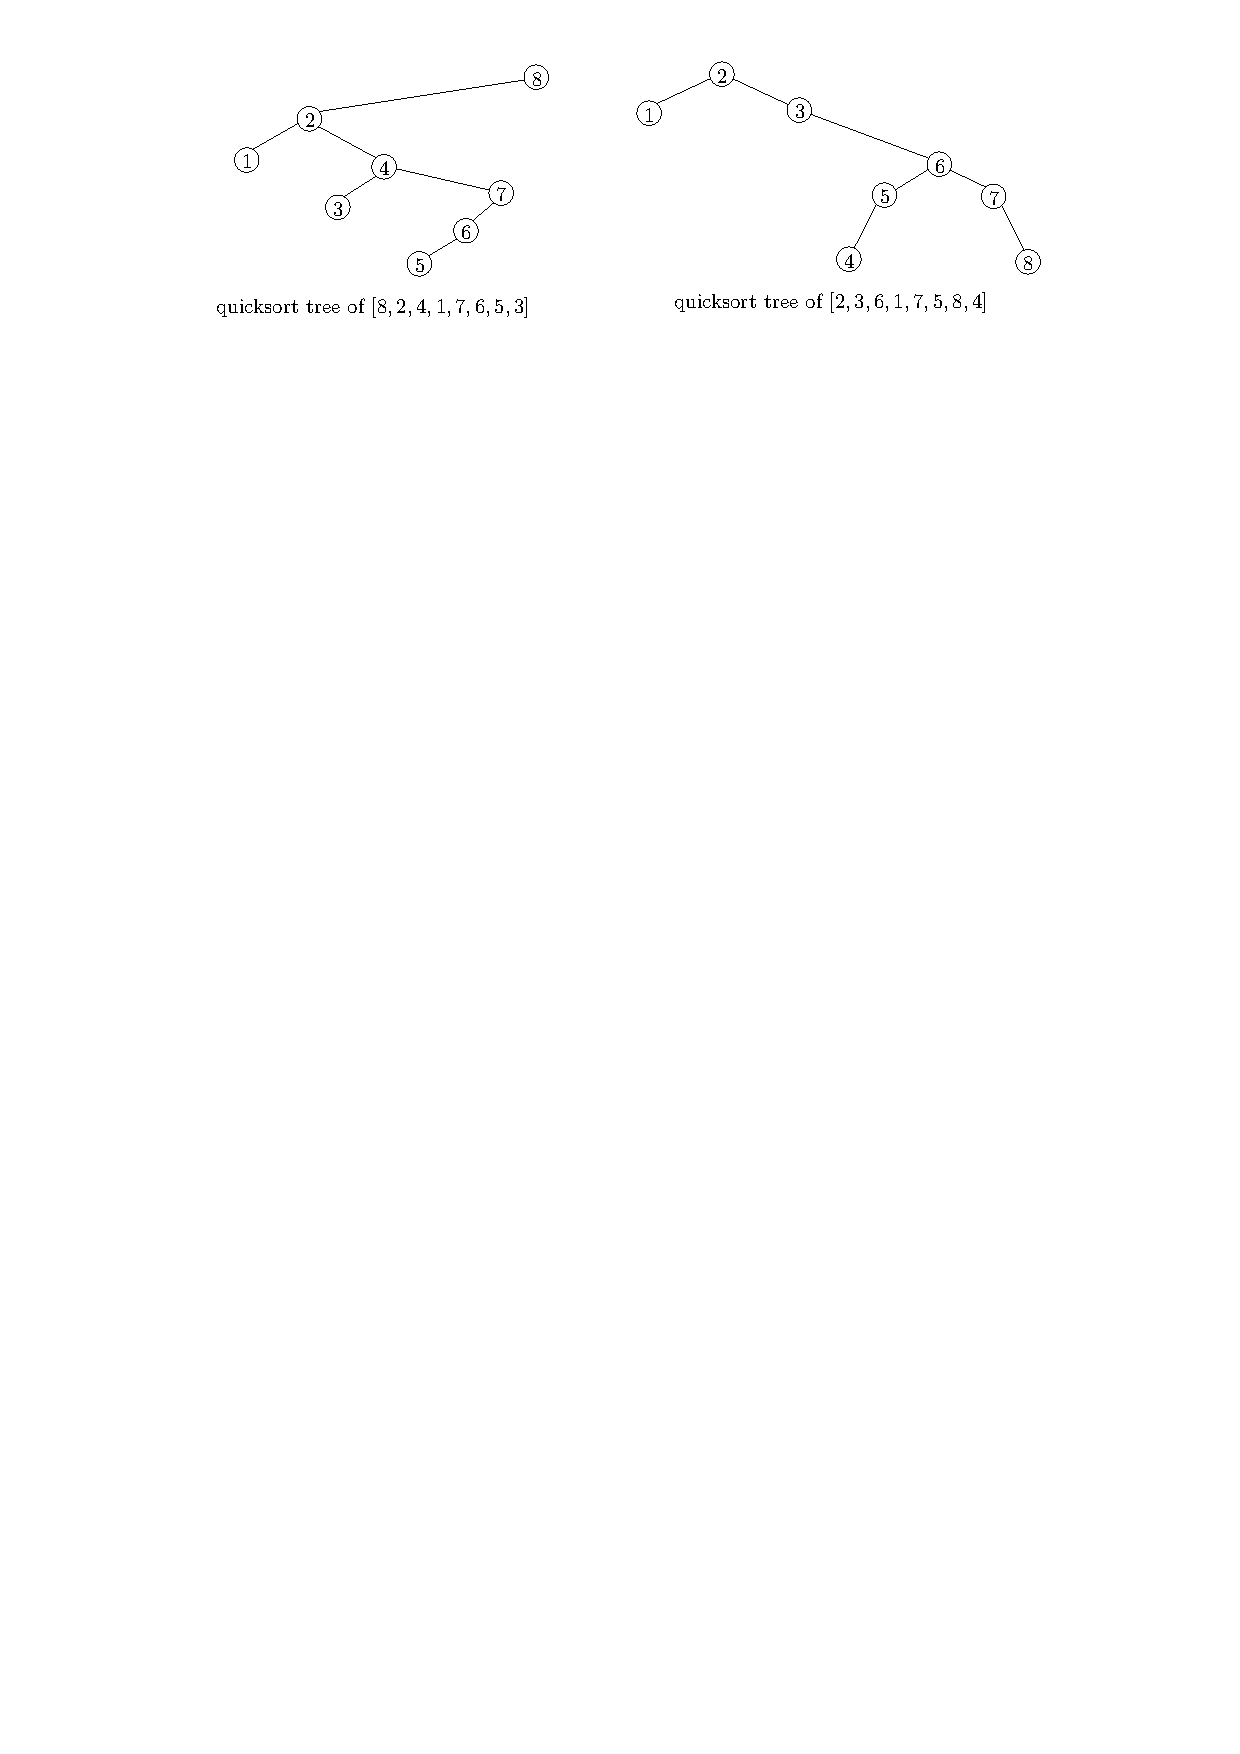
\includegraphics[width=\textwidth]{figures/quicksort-tree.pdf}
\end{center}
\begin{proof}
	For example, if quicksort-tree is left-side tree and k=5, then the visit order of quickselect algorithm is [8, 2, 4, 7, 6, 5]. This is a chain from the root to one of the nodes. Everytime, if the pivot fits the rank we want to find, the result is it. Otherwise, we will recusive the interval fitted the rank what represents the left or right child in quicksort-tree. So, now we get the conclusion: quickselect can be viewed as a "a partial execution" of quicksort with random pivot selection rule.
\end{proof}


Let $B_{i,j,k}$ be an indicator variable which is $1$ if $i$ is a common ancestor
of $j$ and $k$ in the quicksort tree. That is, if both $j$ and $k$ appear in the 
subtree of $T(\pi)$ rooted at $i$.

\begin{exercise}
   What is $\E[B_{i,j,k}]$? Give a succinct formula for this.
\end{exercise}

\begin{proof}
		Similarly, we know that only when $i$ ranks the first in  $[i,j,k]$, can  $i$ be the 
		ancestors of both $j,k$. And the notion means
		 \[
				 [i,j,k]  = \{ \min\left( i,j,k \right) , \ldots, \max\left( i,j,k \right) -1, \max\left( i,j,k \right) \} 
		.\] 
		Hence $\mathbb{E} \left[ B_{i,j,k} \right] = \frac{1}{ \left( \max\left( i,j,k \right) -\min\left( i,j,k \right)  \right) + 1 }$
\end{proof}

\begin{exercise}
  Let $C(\pi,k)$ be the number of comparisons made by \textsc{QuickSelect} when given
  $\pi$ as input. Design a formula for $C(\pi,k)$ with the help of the indicator
  variables $A_{i,j}$ and $B_{i,j,k}$ (analogous to the formula 
  $\sum_{i \ne j} A_{i,j}$ for the number of comparisons made by quicksort).
\end{exercise}

\begin{proof}
		It's easy to find that 
		\[
				C\left( \pi,k \right) = \sum_{i \neq j ,k } B_{i,j,k}
		.\] 
\end{proof}

\begin{exercise}
   Suppose we use \textsc{QuickSelect} to find the minimum of the array. On expectation,
   how many comparisons will it make? Give an answer that is exact up to additive terms 
   of order $o(n)$.
     You can use the fact that $H_k := 1 + \frac{1}{2} + \frac{1}{3} + \cdots  + \frac{1}{n} = \ln(n) + o(1)$.
\end{exercise}

\begin{proof}
		Since $k=1$, we have
		\begin{align*}
				\mathbb{E} \left[ C\left( \pi,k \right)  \right] &= 
				\sum_{i=2}^{n} \sum_{j\neq i} \frac{1}{\max\left( i,j \right) } \\
				&= \sum_{i=2}^{n} \frac{i-1}{i} + \sum_{i=2}^{n} \sum_{j>i} \frac{1}{j} \\
				&= n-2+H_{n} + \left( n-1 \right) H_{n} - \sum_{i=2}^{n} H_{i } \\
				&= nH_{n} + n-1 - \sum_{i=1}^{n} H_{i} \\
				&= nH_{n} + n-1 - \left( \left( n+1 \right) H_{n}-n \right)  \\
				&= 2n-1 - H_{n} = O\left( n \right) -O\left( \log\left( n \right)  \right)  \\
				&=  O\left( n \right) 
		.\end{align*}
\end{proof}
\begin{exercise}
  Derive a formula for $\E_{\pi} [C(\pi,k)]$, up to additive terms of order $o(n)$.
  You might want to introduce $\kappa := k/n$.
\end{exercise}

\begin{proof}
		We need to compute 
		\begin{align*}
				\mathbb{E} \left[ C\left( \pi,k \right)  \right]  &= 
				\sum_{i=1,i\neq k}^{n} \sum_{j\neq i} \frac{1}{\max\left( i,j,k \right) -\min\left( i,j,k \right) + 1} \\
				&= \sum_{i<k} \sum_{j=1}^{n} B_{i,j,k} + 
				\sum_{i>k} \sum_{j=1}^{n} B_{i,j,k} -
				\sum_{i\neq k,j=i} B_{i,j,k} \\
				&= S_1 + S_2 - S_3
		.\end{align*}
		We'll compute the three part one by one
		\[
		S_3 = \sum_{i\neq k} \frac{1}{\lvert k-i \rvert + 1} = H_{k}+H_{n-k+1} -2
		.\] 
		And use the formula $\sum_{i=1}^{n} H_{i} = \left( n+1 \right) H_{n}-n$ we
		have
		\begin{align*}
				S_2& = \sum_{j<k} \sum_{i>k} \frac{1}{i-j+1} +
				\sum_{i>k}\sum_{k\le j\le i} \frac{1}{i-k+1} + \sum_{j>i} \sum_{i>k} \frac{1}{j-k+1}\\ 
				   &=  n-k + \sum_{i>k} \left( H_{i}+H_{n-k+1}-2H_{i-k+1} \right) \\
				   &= 2n-2k+4+\left( k-n-3 \right) H_{n-k+1} + \left( n+1 \right) H_{n}
				   - \left( k+1 \right) H_{k} \\
		.\end{align*}
		Using the same trick we have 
		\begin{align*}
				S_1 &= \sum_{j<i}\sum_{i<k}\frac{1}{k-j+1} + 
				\sum_{i<k}\sum_{i\le j\le k}\frac{1}{k-i+1} + 
				\sum_{j>k}\sum_{i<k} \frac{1}{j-i+1} \\
					&= k-1 + \sum_{i<k}\left( H_{k}+H_{n-i+1}-2H_{k-i+1} \right)  \\
					&= 2k+2 +\left( n+1 \right) H_{n}-\left( k+3 \right) H_{k}
					-\left( n-k+2 \right) H_{n-k+1} \\
		.\end{align*}
		Sum it up, and let $\kappa= \frac{k}{n} $
		\begin{align*}
				S_1+S_2-S_3 &= 2n + 8 + 2\left( n+1 \right) H_{n}
				- \left( 2k+3 \right) H_{k} 
				-\left( 2n-2k+6 \right) H_{n-k+1} \\
							&\approx  O\left( n \right) + 
							2 \left( 
							nH_{n}-kH_{k} - \left( n-k \right) H_{n-k+1} 
							\right)  \\
							&\approx O\left( n \right) + 2n \left( 
							\log n -\frac{k}{n} \log k - \log\left( n-k+1 \right) 
					 + \frac{k}{n}\log\left( n-k+1 \right)   \right)  \\
							&= O\left( n \right)  + 2n\left( 
							\log\left( \frac{1}{1-\kappa+\frac{1}{n} } \right) 
					-\kappa \log\left( \frac{\kappa}{1-\kappa + \frac{1}{n}}  \right)  \right) \\ 
							&= O\left( n \right) + 2\lambda n 
		.\end{align*}
		We only need to consider the size of $\lambda$, since $\kappa \in (0,1]$,  
		and $\frac{1}{n} \to 0$ when $n$ is large
		we have 
		\begin{align*}
				\lambda &= 
				- \left( 1- \kappa \right) \log\left( 1-\kappa \right) - \kappa \log \kappa \\
						&=  - \mathcal{L}\left( \kappa,1-\kappa \right) 
		.\end{align*}	
	 	The form exactly the ML thing which is called \textbf{cross entropy loss}. 
		And we can compute its range by \textbf{Jensen Inequality}: consider 
		$f\left( x \right)  = x\log x$, and $f''\left( x \right) =\frac{1}{x} > 0$.
		And $a+b=1,a,b>0$,  thus 
		\[
				f\left( a \right)  + f\left( b \right)  \ge 
				2f\left( \frac{a+b}{2} \right) = -\log 2
		.\] 
		plus
		\[
				f\left( a \right) +f\left( b \right) < 
				\lim_{x\to 1} \left( f\left( x \right)  + f\left( 1-x \right)  \right)  = 0
		.\] 
		That is $\lambda \in (0, \log 2)$. Which implies that if 
		$\frac{k}{n} = \frac{1}{2}$, we have:
		\[
				\mathbb{E} \left[ C\left( \pi,k \right)  \right] = 
				n\left( 2+\log 2+ O\left( 1 \right)  \right) 
		.\] 
		That is exactly $O\left( n \right) $.
\end{proof}

\end{document}

\subsection{Other Recurrences}

Suppose we are given the recurrence
\begin{align*}
T(n) := \begin{cases}
0 &  \text{if } n \leq 1 \ , \\
 2T(n/2) + n & \text{else.}
\end{cases} \ .
\end{align*}
By looking at the recursion tree, where were able to show that $T(n) \leq n \log(n)$, 
and in fact $T(n) = n \log(n)$ if $n$ is a power of $2$.

\begin{exercise}
   Extend your proof from the previous exercise. Suppose we are given numbers
   $p_1,\dots, p_k \in (0,1)$ such that $p_1 + \cdots + p_k = 1$. Let
\begin{align*}
T(n) := \begin{cases}
0 &  \text{if } n=1 \ , \\
 n +  \sum_{i=1}^k T(p_i n)  & \text{else.}
\end{cases} \ .
\end{align*}  
It is easy to see that $T(n) \in \Theta( n \log n)$, too. However, I want you to determine
the constant factor. That is, determine a number $\gamma$ such that $T(n) = \gamma n \log n + 
o(n \log n)$. \textbf{Remark.} For this, looking at the recursion tree level by level might not be enough. 
You may have to prove it by induction and see for which value of $\gamma$ it ``goes through''.
\end{exercise}



\end{document}